\chapter{Návrh a implementace online nástroje}
\label{chap:design}
U popisování již existujících nástrojů si lze povšimnout toho, že editory jsou svými schopnostmi pokročilé.
Dokáží efektivně pracovat s grafikou a používat různé efekty. Většinu změn lze sledovat v reálném čase. 

Online nástroj, který je součástí této práce by tedy měl mít podobnou funkcionalitu, na kterou jsou obvyklí uživatelé zvyklí.
Těmi mohou být jak zkušení grafičtí designéři, tak i lidé bez hlubší znalosti tvorby bannerů.
Rozsah této práce nepokrývá vytváření grafiky přímo v editoru, a proto bude nástroj koncipován jako prostředek pro využití již vytvořené grafiky.
Prostředí editoru by mělo být reaktivní a reagovat na změny provedené uživatelem.

    \section{Návrh funkcionalit}
    Co se týče práce s textem, měl by být dostupný výběr více fontů, změna barvy, velikosti a podobných možností.
    Na obrázky půjdou aplikovat filtry. Součástí bude taky CTA v podobě tlačítka, které půjde upravovat (šířka, barva, stínování, \ldots) včetně textu uvnitř.
    Transformace, přesouvání a rotace všech objektů je samozřejmostí. Do šablony bude umožněno přidávat více textových objektů a obrázků k
    dosažení požadovaného výsledku. Lze zajistit, aby se některé objekty zobrazovali pouze na vybraných bannerech.

    Tyhle funkcionality umožní vytvoření jakési šablony, ve které budou všechny objekty unikátně pojmenovány.
    Potom uživatel nahraje zdrojový soubor ve formátu CSV, kde každý název sloupce bude odpovídat pojmenovaným objektům.
    Záznamy z CSV souboru jsou dále označovány jako datasety. Na základě dat ze souboru a šablony se vytvoří několik různých setů bannerů,
    které dále půjdou libovolně upravovat nezávisle na sobě. Sloupce odpovídající obrázkům musí obsahovat URL, na kterém je požadovaný obrázek dostupný.

    Výstupem budou exportované bannery ve formátech, které podporují reklamní sítě.
    Snaha bude dosáhnout co nejvyšší kvality při zachování co nejmenší velikosti souborů (max 150 KB). 

    Jelikož tato práce neřeší vzájemný přístup více uživatelů, synchronizace a ukládání pracovního plátna jako takového,
    nebude zde potřeba implementovat serverovou stranu aplikace. Pro funkčnost nástroje lze využít prohlížeč a počítač uživatele.

    % 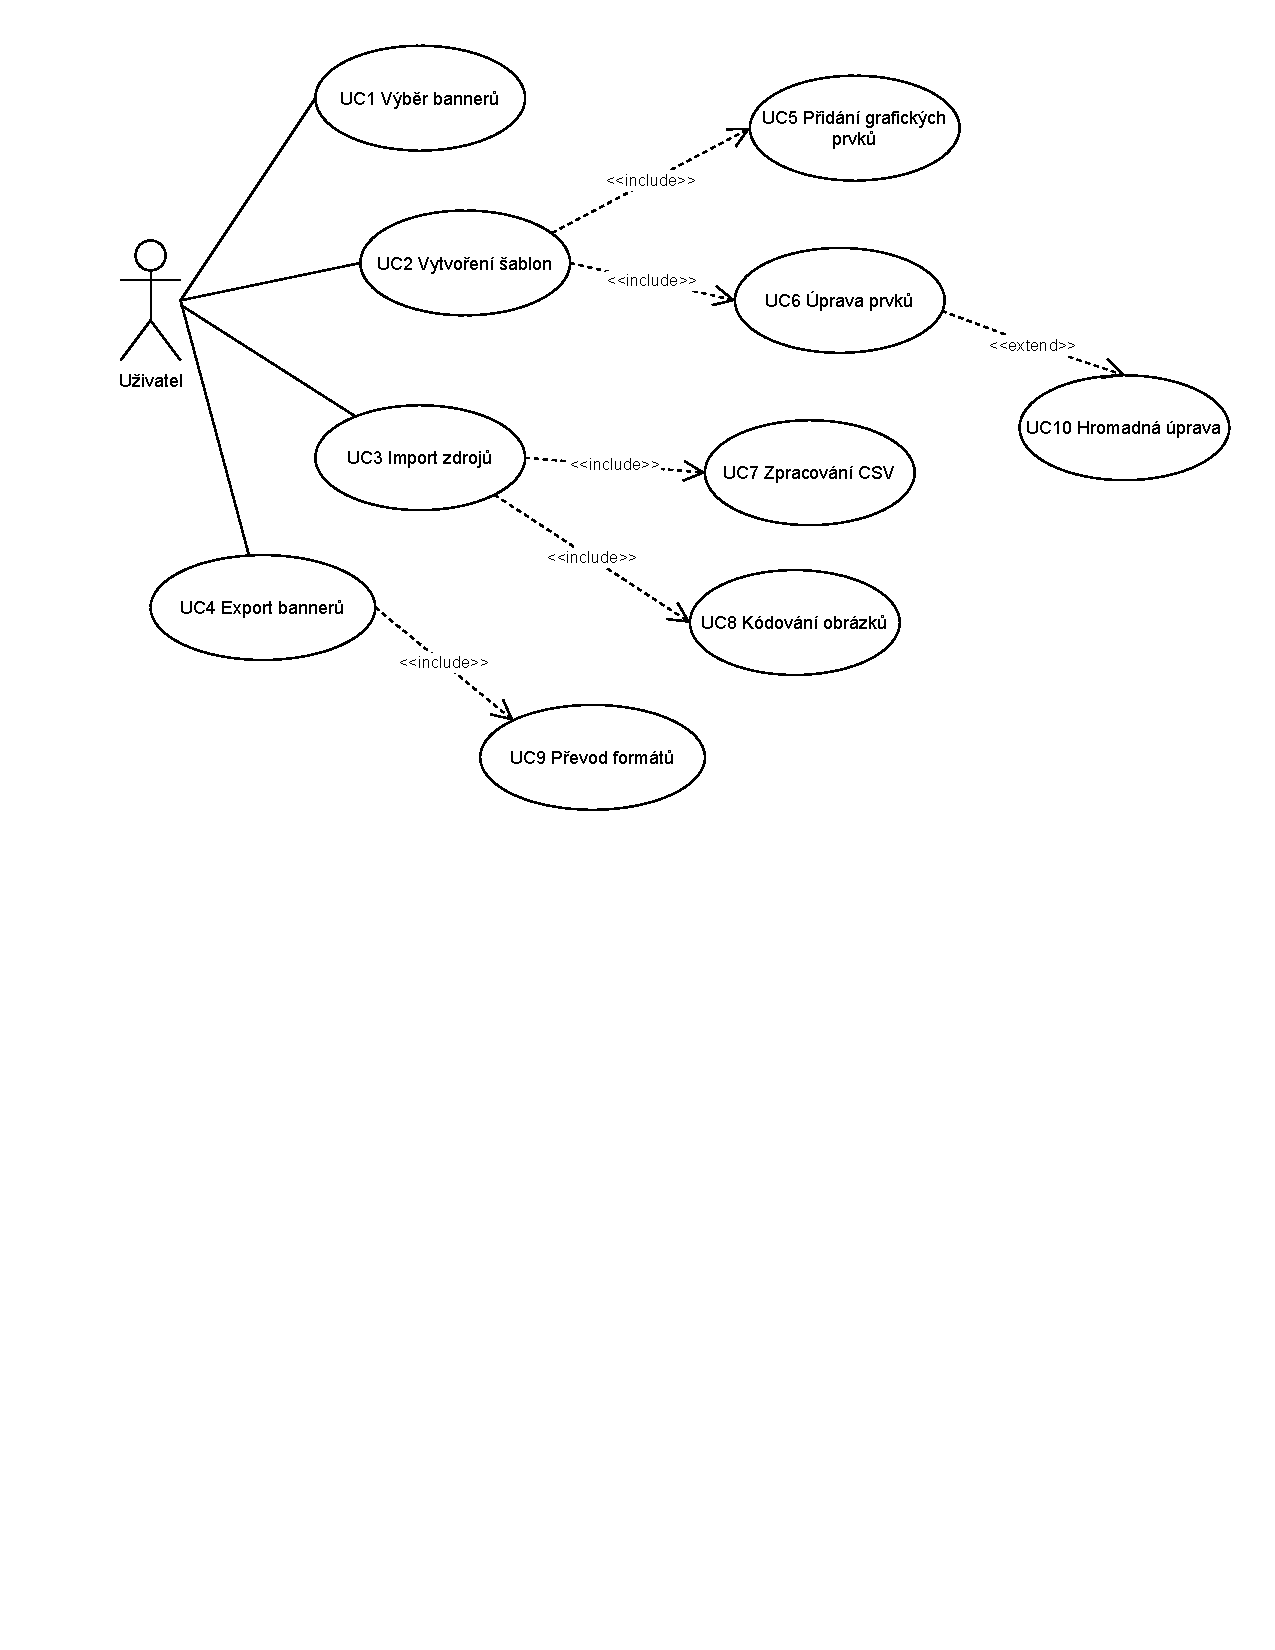
\includepdf{use-case-diagram.pdf}
    %\includesvg{}
    \begin{figure}
        \centering
        \label{fig:use-case-diagram}
        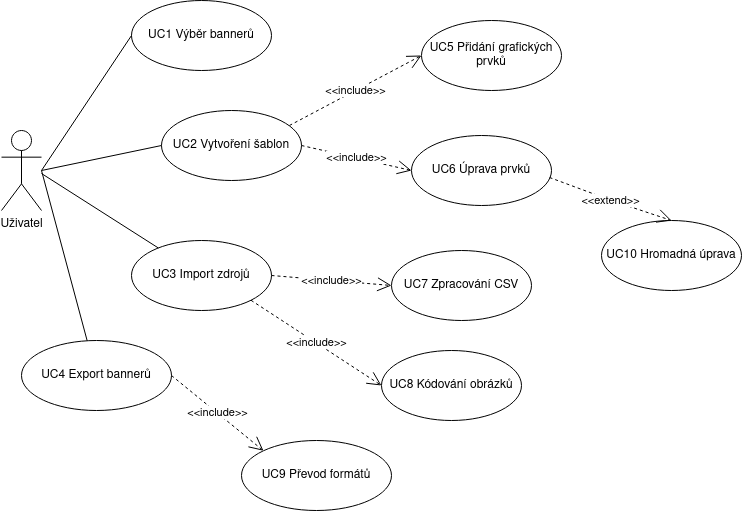
\includegraphics[width=0.85\textwidth]{Figures/use-case.png}
        \caption[Use case diagram]{Diagram případu užití návrhu online nástroje}
    \end{figure}

    \section{Volba technologíí}
    Moderní vývoj frontendu se ujal směrem javascriptových frameworků a knihoven. Nejvíce používanými frameworky/knihovnami se stal VueJS, Angular a React.
    Porovnávat tyto technologie by však bylo zbytečné zde rozepisovat, jelikož to není tématem této práce.
    Pro případný zájem autor doporučuje tento článek, kde jsou většina porovnání včetně benchmarků.
    Nutno podotknout, že zatímco React a Vue jsou zaměřené více na hlavní funkcionalitu a ostatní věci jako routování a state management nechávají
    na dodatečných balících. Angular většinu funkcí obsahuje v základu.
    I z tohoto důvodu a lepší znalosti frameworku Angular se autor této práce rozhodl právě pro tuto možnost. 

    Pro práci grafikou na straně prohlížeče jsou k dispozici 2 HTML elementy a tím jsou Canvas a SVG.
    Canvas, v překladu kreslící plátno, kreslí použitím rastrové grafiky. Oproti tomu SVG je kreslí vektorovu grafiku.
    Jelikož je cílem práce tvorba bannerů, do kterých má být možno vkládat fotografie, padá volba na Canvas.
    Samotný canvas ale neposkytuje moc rozšířenou funkcionalitu. Naštěstí na tento problém existuje řešení v podobě knihoven.

        \subsection{JS knihovny pro práci s Canvas elementem}
        Javascriptový ekosystém je velice rozsáhlý a je z čeho vybírat. Dostupných knihoven pro práci s canvasem je mnoho.
        Ne každá knihovna ale poskytuje potřebnou funkcionalitu,
        jelikož se zaměřuje na jiný problém. Tato část porovná pár autorem vybraných knihoven.

            \subsubsection{Fabric.js}
            První porovnávanou knihovnou je Fabric.js. Dokáže pracovat s jakýmkoli tvarem nebo vloženým obrázkem. Umožňuje na obrázky používat filtry,
            má zabudovanou podporu tvorby animací, seskupování objektů a stínování. Poradí si i při práci s textem, se kterým dokáže vykreslovat různé fonty,
            zarovnávat jej a samozřejmě měnit velikost.
            Výhodou této knihovny oproti ostatním je, že má zabudovaný parser pro konverzi do formátu SVG nebo JSON a zpět z těchto na canvas.  
            
            \subsubsection{Konva.js}
            KonvaJS je knihovna pro práci ve 2D jak pro desktopové zařízení, tak pro mobilní. Nabízí práci s textem (včetně podpory různých fontů),
            animace, geometrickými objekty, obrázky (rastrové i vektorové) a videa, filtry atd. Výsledek práce se dá exportovat jako serializovaný
            JSON nebo obrázek ve formátu PNG nebo JPEG, u kterých umožňuje zvýšit poměr pixelů pro lepší kvalitu.
            Při exportu do formátu JPEG dovoluje zvolit výslednou kvalitu. Mezi výhody spadá podpora zařízení s vysokou hustotou pixelů, a gest na mobilních zařízeních.
            Pro programátory nabízí i statické typování v podobě definicí v Typescriptu. 

            \subsubsection{Easeljs}
            Tato knihovna jako předešlé disponuje velkou škálou funkcionalit.
            Oproti ostatním ale nemá přímo zabudovanou možnost animací.
            Podporuje mobilní zařízení a do jisté míry vykreslování pomocí technologie WebGL.

            Jelikož je vysoká pravděpodobnost, že by nástroj používali grafici, je potřeba zajistit dobrou podporu pro retina displeje.
            Proto pro implementaci byl zvolena KonvaJS.

    \section{Návrh implementace}
    Základním stavebním blokem aplikací v Angularu jsou moduly. Ty logicky oddělují různé části aplikace od sebe a tím umožňuje lepší oddělení
     zodpovědností (Separation of concerns). Další 2 hlavní prvky, které pomohou k implementaci jsou komponenty a služby.  

    Komponenty spravují viditelné části uživatelského rozhraní a jejich interakci s uživatelem (vstupy, události).
    Vazba mezi viditelnými částmi HTML a komponentami je obousměrná. Díky tomu se všechny prvky rozhraní aktualizují na základě momentálního stavu aplikace,
    který je uživateli zobrazen a zároveň reaguje na jeho podněty. Navíc, komponenty lze znovu využívat a dávat jim vstupní parametry.
    Tato výhoda bude použita pro zobrazení úprav více objektů stejného typu. 

    Služby naopak slouží pro zachycení funkcionalit, které typicky nemají souvislost s uživatelským a mohou být opakovaně použity napříc aplikací.
    Přístup ke službám je zajištěn přes dependency injection (injektáž závislostí, DI). Lze je injektovat do komponent nebo ostatních služeb.
    Důležité je vědět, že injektace probíhá skrz tzv. providery. Ti říkají, v rámci čeho je služba poskytována (modul, komponent, aplikace) a
    podle toho vytvářejí instance. Jelikož vstupů, které budou ovlivňovat vykreslování bannerů na plátně bude hodně,
    byla by komunikace striktně mezi komponentami složitá. Proto bude využita sdílená služba.
    Ta má za úkol zastiňovat API vybrané knihovny a vykreslování na plátno. Díky tomu budou mít všechny potřebné komponenty přístup ke službě a
    přímo ovlivňovat vykreslené objekty.

    \begin{figure}[h]
        \centering
        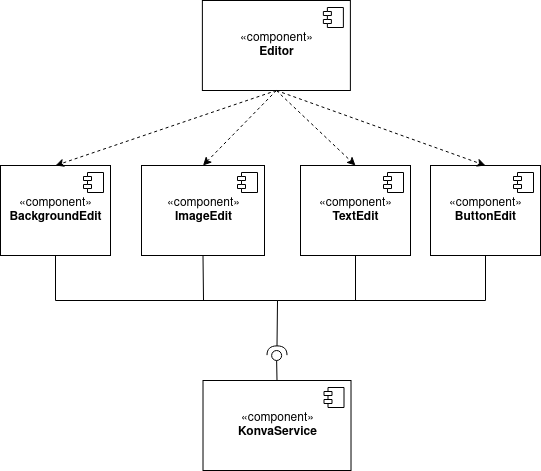
\includegraphics[width=0.85\textwidth]{Figures/component-diagram.png}
        \label{fig:component-diagram}
        \caption[Diagram komponent editoru]{Diagram komponent online nástroje}
    \end{figure}

        \subsection{Zobrazení více bannerů najednou}
        Aby uživatel dokázal pracovat rychle a efektivně bude mu umožněno upravovat více bannerů najednou. K docílení tohoto požadavku je možno použít
        třídu \emph{Konva.Group}. Ta umožňuje seskupení vícero objektů a jejich oříznutí.
        Každá skupina bude reprezentovat jeden banner. Oříznutím bude zajištěno zobrazení, indikující přesah okraje banneru.

        \subsection{Práce s tvary na plátně}
        Práce s tvary jako přesouvání a transformace jsou základem grafických editorů. Díky použité knihovně zajištění těchto funkcí nebude složité.
        Ale potřebou je, aby se provedená transformace projevila i na ostatních bannerech. Pro implementaci transformací lze využít třídu \emph{Konva.Transformer}.
        Ta mimo jiné poskytuje události \emph{transformstart, transform, transformend}, díky kterým bude jasné, co se s objektem děje a aplikovat stejnou transformaci i
        na stejné objekty v ostatních bannerech. Stejný postup platí i pro rotaci.

        Při přesouvání nastává událost \emph{dragmove}. K té také lze naslouchat. Naivní možnost by byla přesouvat na ostatních bannerech stejný tvar o počet pixelů,
        o které byl posouvaný tvar změněn. To ale způsobí, že na malých rozměrech by se objekt dostal rychle na hranici a na velkých rozměrech by
        změna nešla skoro poznat. Při přesouvání se musí vzít v potaz velikost přesouvaného objektu a zároveň rozměr banneru, na kterém má být přesunut.
        Jako možnost se nabízí spočítat si pozici středu objektu v procentech v závislosti na daném banneru.
        Potom si pozici pro příbuzné objekty jde snadno dopočítat.

        Pro pozicování pozadí v případě, že půjde o obrázek, bude použité jiné chování přesouvání. Místo toho, aby se vykresloval celý, bude vykreslován jen výřez.
        Pokud bude nutné zobrazit na pozadí jinou část obrázku, potáhnutím pozadí lze měnit pozici výřezu, který bude vykreslen.

        Při různých úpravách se však může stát, že některé objekty se na bannery menších rozměrů nevlezou nebo budou muset být jinak upraveny.
        Proto bude umožněno je odebrat nebo individuálně upravit.

        \subsection{Úpravy textu}
        ext je na banneru velice důležitý. Z tohoto důvodu by měla editace textu nabízet obvyklé prvky jako výběr fontu.
        Pro možnost širokého výběru bude zajištěno napojení na Google Fonts a tím i zpřístupněny všechny fonty, jenž Google poskytuje.
        Dále pro text budou možnosti jako je zarovnání textu, zalamování, kurzíva, tučný text, změna barvy a stínování pod textem.
        Vykreslování stínů na canvasu v prohlížeči je výpočetně složitá operace. K urychlení lze použít schopnost knihovny Konva.js uložení v mezipaměti,
        což převede celý text i se stínem na obrázek,
        který je jednodušší vykreslit. Při následné jakékoliv změně textu se mezipaměť přepíše novými hodnotami.

        \subsection{Nahrávání obrázků}
        Cílem je práci usnadnit co nejvíce a umožnit nahrání jak ze vzdálených zdrojů, tak i z lokální pracovní stanice.
        Obvykle by se obrázky a fotografie nahráli na server, odkud by již byly dostupné uživateli kdykoli by je potřeboval.
        Tohle jsou však další rozšířené funkce, které tato práce svým rozsahem neřeší. Proto bude nahrávání řešeno pomocí kódování base64,
        které umí binární data převést na ASCII znaky. Tento přístup je nutné použít i v případě nahrání ze vzdálených zdrojů Internetu.
        Dle specifikace HTML, načítání obrázků z jiné domény do canvasu způsobí tzv. zkažený (tainted) canvas, který není možné exportovat.
        Další způsob je povolení \emph{CORS} ze strany zdrojového serveru. Díky tomu by se obrázky mohli načíst bez nutnosti kódování.

        \subsection{Exportování výsledků}
        Stejně jako nativní HTML canvas, Konva.js poskytuje možnost exportování ve formátech JPG a PNG.
        Výsledek za zakódován v base64, který už však není problém zobrazit nebo stáhnout.
        Není potřeba však exportovat celé pracovní plátno, ale jen potřebné bannery. Ty, jak je již bylo zmíněno,
        jsou pouhým seskupením různých objektů. Pro zařízení s vyšší hustotou pixelů je dostupná možnost exportovat se zvýšeným poměrem pixelů (pixel ratio). 

        Zde ovšem je potřeba zajistit, aby výsledný export byl v co nejvyšší kvalitě a zároveň nejmenší velikosti.
        Preferovaný formát při exportu bude PNG, jelikož je bezztrátový. Pokud by výsledný soubor přesahoval 150 KB,
        další možností je použít 24bitový formát PNG-24.
        Ten neuchovává informace o průhledném alfa kanálu a tím na každý pixel ušetří 1 bajt, celkově tedy je možná úspora až 25\% původní velikosti. 

        Alternativou k těmto formátům je nový formát speciálně vytvořený pro web. Tím je formát WebP, vyvíjený společností Google.
        Dle oficiálních zdrojů podporuje ztrátovou i bezztrátovou kompresi. Přičemž v porovnání v PNG dokáže smrsknout až o 26\% lépe a v porovnání
        s JPEG dokonce až o 34\%. Podpora zobrazení tohoto formátu je rozšířená na všechny nejvíce využívané webové prohlížeče.
        Kromě Facebooku, stále mnoho reklamních systémů, včetně Googlu samotného, tento formát nepodporuje.

        \subsection{Ukládání projektu}
        Projekt se všemi úpravami půjde uložit do souboru. Ten bude obsahovat potřebná data ke znovuvytvoření identické stavu, jako byl před uložením.
        Díky této funkci uživatelé nepřijdou o veškerý postup, který udělali.

    \section{Datové struktury}
    Při nahrávání datasetů je potřeba nějakým způsobem uložit nahraná vstupní data. Jelikož online editor musí být schopný upravovat šablonu i dataset,
    musí se pro každý objekt na plátně ukládat i jeho stav. V každém datasetu budou uchovávány informace o bannerech, které se mají vykreslit.
    A pro každý banner musí být uložen momentální stav jednotlivých objektů. Tohoto lze docílit serializací vykreslených uzlů.
    Konva.js se serializací tvarů počítá, a proto ukládá pouze změněné vlastnosti. V případě budoucího rozšíření, by bylo vhodné taková data ukládat spíše do
    dokumentových NoSQL databází jako je například MongoDB a využít tak možnosti vnořených kolekcí dokumentů. 

    Uchováváním těchto dat v paměti bude zajištěno, že každý banner v jakémkoli datasetu bude moct být opětovně správně vykreslen.

    \section{Návrh uživatelského rozhraní}
    Rozhraní grafických editorů musí být intuitivní. Podobné nástroje už existují dlouhou dobu a jejich uživatelé mohou být zvyklí na pojmenování určitých funkcí
    nebo znázornění ikonkou. Proto je třeba, aby i implementovaný nástroj se vzhledem blížil nebo podobal zavedenému de facto standardu grafických editorů. 

    Součástí prostředí bude horní lišta. Ta bude mít na levé straně tlačítko pro hlavní nabídku. Součástí nabídky budou položky pro:
    \begin{itemize}
        \item export všech bannerů,
        \item uložení do souboru.
    \end{itemize}
    Na pravé straně lišty půjdou najít možnosti lokalizace. Implementace nástroje v rámci této práce bude lokalizována do 2 jazyků. Těmi jsou čeština a angličtina. 

    Editor bude mít 2 postranní sloupce mezi kterými se bude nacházet pracovní plátno. Levý sloupec bude obsahovat seznam šablon,
    které se budou moct přehazovat a přejmenovávat. Vedle seznamu také budou dostupné některé základní nástroje pro kreslení tvarů.
    Na pravém sloupci budou zobrazeny všechny tvary a objekty, které se momentálně nachází na bannerech, po položkách.
    Jednotlivé položky půjdou rozkliknout a zobrazí se vlastnosti objektu, jenž půjdou změnit.

    \begin{figure}[ht]
        \centering
        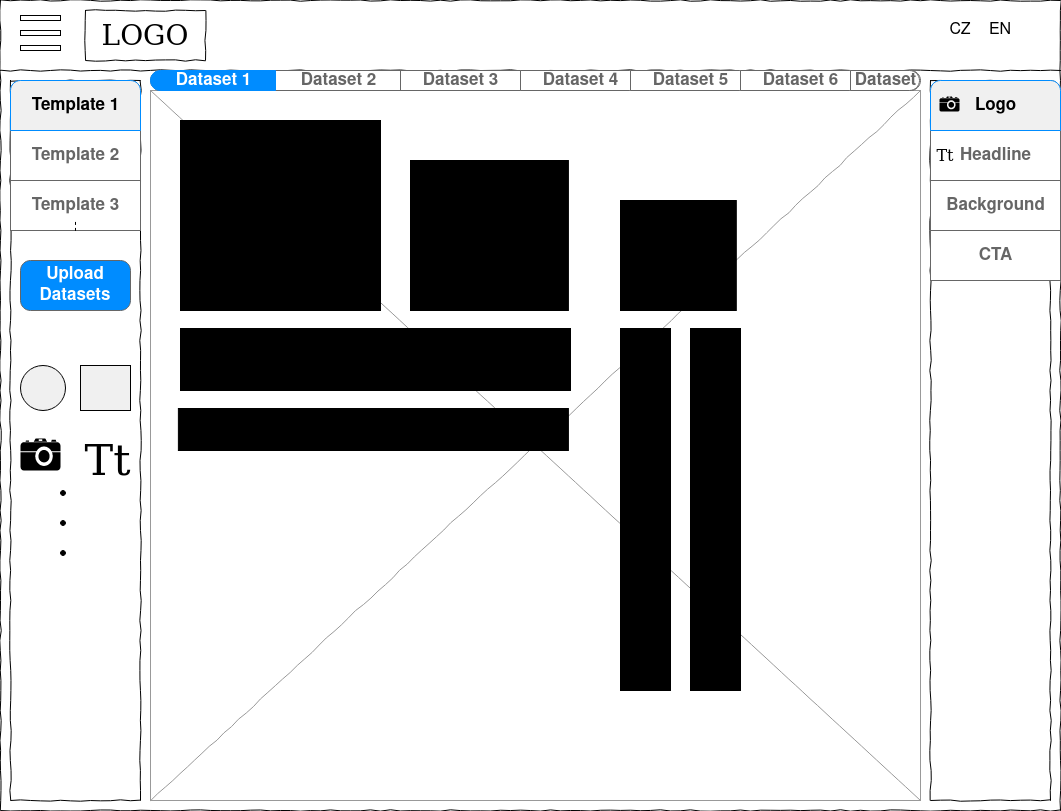
\includegraphics[width=0.8\textwidth]{Figures/wireframe.png}
        \label{fig:ui-wireframe}
        \caption[Wireframe UI]{Návrh uživatelského rozhraní ve formě wireframu}
    \end{figure}

        \subsection{Text}
        Výběr fontů bude implementován způsobem vyhledávání s automatickým zobrazením nebližších shod.
        Textové sdělení jako takové půjde vložit přes textovou oblast. Barva bude vybírána skrze samostatnou komponentu, kde barva půjde zadat buďto
        ve složkách RGB nebo jako HEX řetězec nebo bude moct být vybrána. K barvě je i možný alfa kanál.
        Zarovnání textu, ztučnění, kurzíva, podtržení a přeškrtnutí budou jednoduchá tlačítka, která budou indikovat, zda jsou aktivní nebo ne,
        a to změnou pozadí. Výška řádku a mezera mezí písmeny budou měnitelné přes posouvátko.

        \subsection{Obrázkové filtry}
        Jelikož u některých filtrů jde změnit \enquote{síla} účinnosti (např. kontrast, zesvětlení, posterizace, \ldots), bude možné ji měnit jako posouvátko.
        Ostatní filtry, které mají stav pouze vypnuto/zapnuto (invertování barev, stupně šedi), bude možno aktivovat pomocí přepínače.

        \subsection{CTA}
        Tlačítko pro vyzvání k akci je kombinací textu a jednoduchého tvaru na pozadí. Stylizace bude rozdělena na 2 záložky, kde jedna je pro úpravu textu a
        druhá pro úpravu pozadí. Pro CTA bude možnost zaoblení rohů.

        \subsection{Export}
        Exportování výsledků bude provedeno v rámci dialogového okna v krocích, které postupně navedou uživatele.
        Prvním krokem bude výběr výsledného formátu. V případě, že bude jednat o JPEG, zobrazí se i volba nejvyšší možné kvality.
        Druhý krok bude výběr datasetů k exportu, ze kterých půjdou vybrat třeba jen určité bannery. Třetím a zároveň posledním krokem je
        samotné stažení bannerů v archivu. 




\endinput